% controlled fusion and RF heating and current drive
%\chaptertoc{}

\chapter{Controlled Fusion, RF heating and Current Drive}
\label{chap:fusion_and_rf}
\margintoc

%%%%%%%%%%%%%%%%%%%%%%%%%%%%%%%%%%%%%%%%%%
%%%%%%%%%%%%%%%%%%%%%%%%%%%%%%%%%%%%%%%%%%
\section{Nuclear Fusion}
\subsection{Fusion Power}
\marginnote{Part of this section are taken from Master Fusion lecturer notes on Tokamak dimensioning, from which the paper \citeauthyear{sarazin2019} has been derived.}

Nuclear fusion is the process that powers all the stars in the Universe, including our Sun. If controlled in a reactor, fusion power could be an ideal energy source. It would run on hydrogen isotopes\sidenote[][*+3]{Such as deuterium which can be found in sea water and tritium which can be generated inside the reactor}, does not generate greenhouse gas and creates no radioactive waste except the reactor vessel components itself. It would be a dispatchable source (in contrast to intermittency inherently affecting solar and wind energies) and would require much less land area than wind or solar power installations for similar power. But producing a self-sustaining fusion reaction requires that deuterium and tritium be heated to over 150~million~\si{K}, a temperature at which they become plasma: an electrically charged gas. 

Indeed, to get nuclear fusion, nuclei have to come close enough to each other where nuclear forces can overcome their mutual electrostatic repulsion. This would require temperatures of the order of 720 \si{keV} for head-on collisions of thermal particles to lead to fusion reactions in a classical way. 

Actually, quantum physics has to be taken into account in the process. Both in tokamaks and in stars interiors, fusion reactions take place predominantly due to the tunnel effect. Crossing this barrier can be quantified in a probabilistic manner with the \textit{reaction rate} $r$ $[\si{reaction/(m^3.s)}]$, defined as the probability of reaction per unit time and volume. 
The reaction rate between mono-energetic ions "1" of density $n_1$ $[\si{m}^{-3}]$ striking target ions "2" of density $n_2$ $[\si{m}^{-3}]$ is proportional to the effective cross-section area $\sigma_{12}$ $[\si{m}^2]$ and to the velocity difference $v_{12}$ between the two species:
\begin{equation*}
	r_{12} = n_1 n_2 \; \sigma_{12} v_{12}
\end{equation*}
The quantity  $\sigma_{12} v_{12}$, which depends on the kinetic energy of the colliding particles, is called the \textit{reactivity} ($\mathrm{[m^3/s]}$). The reaction rate $r_{12}$ is proportional to the square of the density of the mixture. In fusion plasmas, ions are not mono-energetic, they are assumed to have Maxwellian velocity distributions. The average reactivity $\langle \sigma_{12} v \rangle_{12}$ derives from the following expression:
\begin{equation*}
	\left < \sigma v \right >_{12} 
	= \int_{-\infty}^{+\infty} \int_{-\infty}^{+\infty} 
	\sigma(v_{12}) v_{12}\;  f_1(v_1) f_2(v_2) \; dv_1dv_2
\end{equation*}

Finally, the average reaction rate $\left < r_{12} \right >$ reads:
\begin{equation*}
	\left < r_{12} \right > = n_1 n_2 \; \left < \sigma v \right >_{12}
\end{equation*}
The temperature dependence of the reactivity $\langle \sigma v \rangle_{12}$ is plotted on figure~\ref{fig:chap1:reactivity} for several fusion reactions.

\begin{figure} 
	\begin{center}
		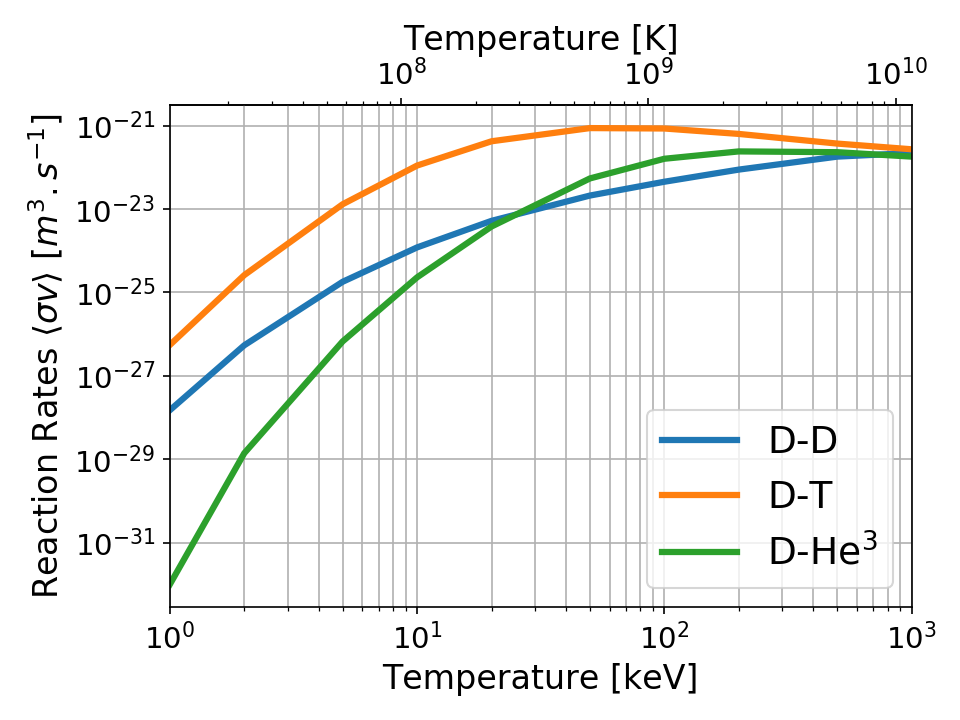
\includegraphics[width=1.0\textwidth]{figures/chap1/Fusion_Reactivity.png}
		\caption{Fusion reactivity versus temperature for few couples of fusion reactions. Data from \citeauthyear{richardson2019}.}
		\label{fig:chap1:reactivity}
	\end{center}
\end{figure}

From Figure~\ref{fig:chap1:reactivity}, the Deuterium (D)-Tritium (T) reactivity $\left<\sigma v\right>_{\mathrm{DT}}$ reaches its maximum for a temperature of 64 keV, corresponding to a temperature of $742\,10^6$ K. Since it has the highest reaction rate, the D-T reaction is the “easiest” to initiate (maximum reactivity at lowest temperature) of all fusion reactions and is the main targeted reaction for controlled fusion reactors\sidecite{cea1987, ball2019}: 
\begin{equation}
	\mathrm{D + T} \longrightarrow \mathrm{{}^4 He~(3.56~MeV) + n~(14.03~MeV)}
\end{equation}

The D-T reaction leads to a total released energy of $E_{DT}$ = 17.59~\si{MeV} = $2.82\times 10^{-12}$~\si{J} per fusion reaction, where almost 80\% of the energy is carried by the neutrons\sidenote{This value can be compared to the 200~MeV released by $^{235}$U fission. Yet, the energy release \emph{per nucleon} ($i.e.$ per kilogram) is approximately 4 times larger for fusion than for fission reactions.}. Assuming equal deuterium and tritium densities $n_D = n_T = \frac{n}{2}$, with $n$ the electron density, then the thermonuclear power density reads:

\begin{equation}
p_{\mathrm{DT}} = 
	\frac{n^2}{4}  \left< \sigma v \right>_{\mathrm{DT}} E_{\mathrm{DT}}
	\label{eq:fusion_power}
\end{equation}

The total fusion power $P_{\mathrm{fus}}=\int p_{\mathrm{DT}} \diff V$ is distributed among the alpha particles and the neutrons: 
\begin{equation}
P_{\mathrm{fus}}
= 
P_\alpha + P_n 
\doteq
\lambda \; P_\alpha
\label{eq:P_fus_Palpha}
\end{equation}
where we defined $\lambda = 17.59/3.56 \approx 4.94$ for a reason which will be clear in the next section.


%Assuming a constant reactivity in the plasma ("flat profile hypothesis") and using the tore volume $V$, the fusion power is: 
%\begin{equation}
%P_{fus} = \frac{V}{4}
%n^2 \left< \sigma v \right>_{DT} E_{DT}
%\end{equation}
%
%For a circular cross-section, the plasma volume is $V=2\pi^2 R a^2$. The reactivity $\left< \sigma v \right>_{DT}$ depends on the temperature. In the temperature range 10.3-18.5 keV, it turns out that the reactivity $\left< \sigma v \right>_{DT}$ can well (with about 10$\%$ error) be approximated by \sidecite{wesson2011}: 
%\begin{equation*}
%	\left< \sigma v \right>_{DT} \approx 1.18\, 10^{-24}\; \hat T^2 \;\si{\left[m^3 s^{-1}\right]}
%\end{equation*}
%where $\hat T$ is expressed in $\si{keV}$.

%%%%%%%%%%%%%%%%%%%%%%%%%%%%%%%%%%%%%%%%%%
\subsection{Triple Product}
At equilibrium in a fusion power plant, sources terms equal loss terms:
\begin{equation}
	\sum_{\mathrm{sources}} P = \sum_{\mathrm{loss}} P
	\label{eq:power_balance_general}
\end{equation}

To the contrary with neutrons which leave the plasma, charged $\alpha$~nuclei are confined by the magnetic field and should ideally transfer their energy to the main ions before being extracted\footnote{There are basically 2 ways for this energy transfer. Since the collision frequency scales like the velocity difference between the colliding species to the power $-3$ ($\nu_{coll,ss'}\sim n_{s'}/\Delta v_{ss'}^3$), alpha particles transfer their energy dominantly to the electrons, which are much faster due to their low inertia. Then two routes are possible for the energy transfer from the electrons to the ions. Either via collisions, or via turbulence. In the latter case, the mediator are the electrostatic plasma waves. The relative weight of those two channels is still a matter of research.}. The source term is the sum of the plasma heating $P_{H}$ mechanisms and of alpha heating $P_\alpha$:

\begin{equation}
\sum_{\mathrm{sources}} P
	\doteq 
	P_\alpha + P_{H} 
	\label{eq:sources}
\end{equation}

The losses origins being diverse, it is convenient to separate losses into thermal transport losses $P_{\mathrm{cond}}$ (conduction and convection) and radiative losses $P_{\mathrm{rad}}$\sidecite{wesson2011}. Usually, the energy confinement time $\tau_E$ ([\si{s}]) is defined as the characteristic time at which the total thermal plasma energy $W=3 n k_B T$ is lost to its environment, either by collisional conduction or by turbulent thermal convection:

\begin{equation}
\sum_{\mathrm{loss}} P 
	=
	P_{\mathrm{cond}} + P_{\mathrm{rad}}
	\doteq 
	\frac{ W }{ \tau_E } + P_{\mathrm{rad}}
	\label{eq:losses}
\end{equation}
Thus, at the equilibrium, power conservation leads to:
\begin{equation}
P_\alpha + P_{H} = \frac{ W }{ \tau_E } + P_{\mathrm{rad}}
\end{equation}
Keeping only conduction losses and ignoring radiation loss (which is a large approximation) and assuming the plasma is mainly heated by $\alpha$ particles ($P_H\ll P_\alpha$), Lawson\sidecite{lawson1957} estimated a criteria for which fusion power exceeds the losses, which leads to the following criteria (or "triple product"):
\begin{equation*}
	P_{\mathrm{fus}}/\lambda > \frac{3n k_B T}{\tau_E}
	\Rightarrow
	n \tau_E T > 
		\frac{12 \lambda k_B}{E_{\mathrm{DT}}} 
		\frac{T^2}{\left<\sigma v \right>_{\mathrm{DT}}}
\end{equation*}
As illustrated in Figure~\ref{fig:chap1:reactivity}, the reactivity $\left<\sigma v \right>_{\mathrm{DT}}$ depends on the temperature. The quantity $T_i^2 / \left<\sigma v \right>_{\mathrm{DT}}$ is found to have an absolute minimum around 14 $\si{keV}$. In this temperature region, the D-T reactivity can be approximated as $\left<\sigma v \right>_{\mathrm{DT}}\approx 1.1\times10^{-24} \hat{T}^2$~\sidecite{wesson2011,cea1987}. 
\marginnote[*+2]{$\hat T$ is expressed in \si{keV}: $\hat T=10^{-3} k_B T_{[K]}/e$}
This leads to:
\begin{equation}	
	n \hat{T} \tau_E > 3\times 10^{21} \, \si{keV.s.particles/m^3}
	\label{eq:lawson_criteria}
\end{equation}
Past or current fusion reactors achieved so far 1/10th of this value, but 30 years ago they only achieved 1/100 000th of it. Some of these performances are illustrated for various present and future magnetic confinement devices in Figure~\ref{fig:chap1:nTtau_machines}.



\begin{figure} 
	\begin{center}
		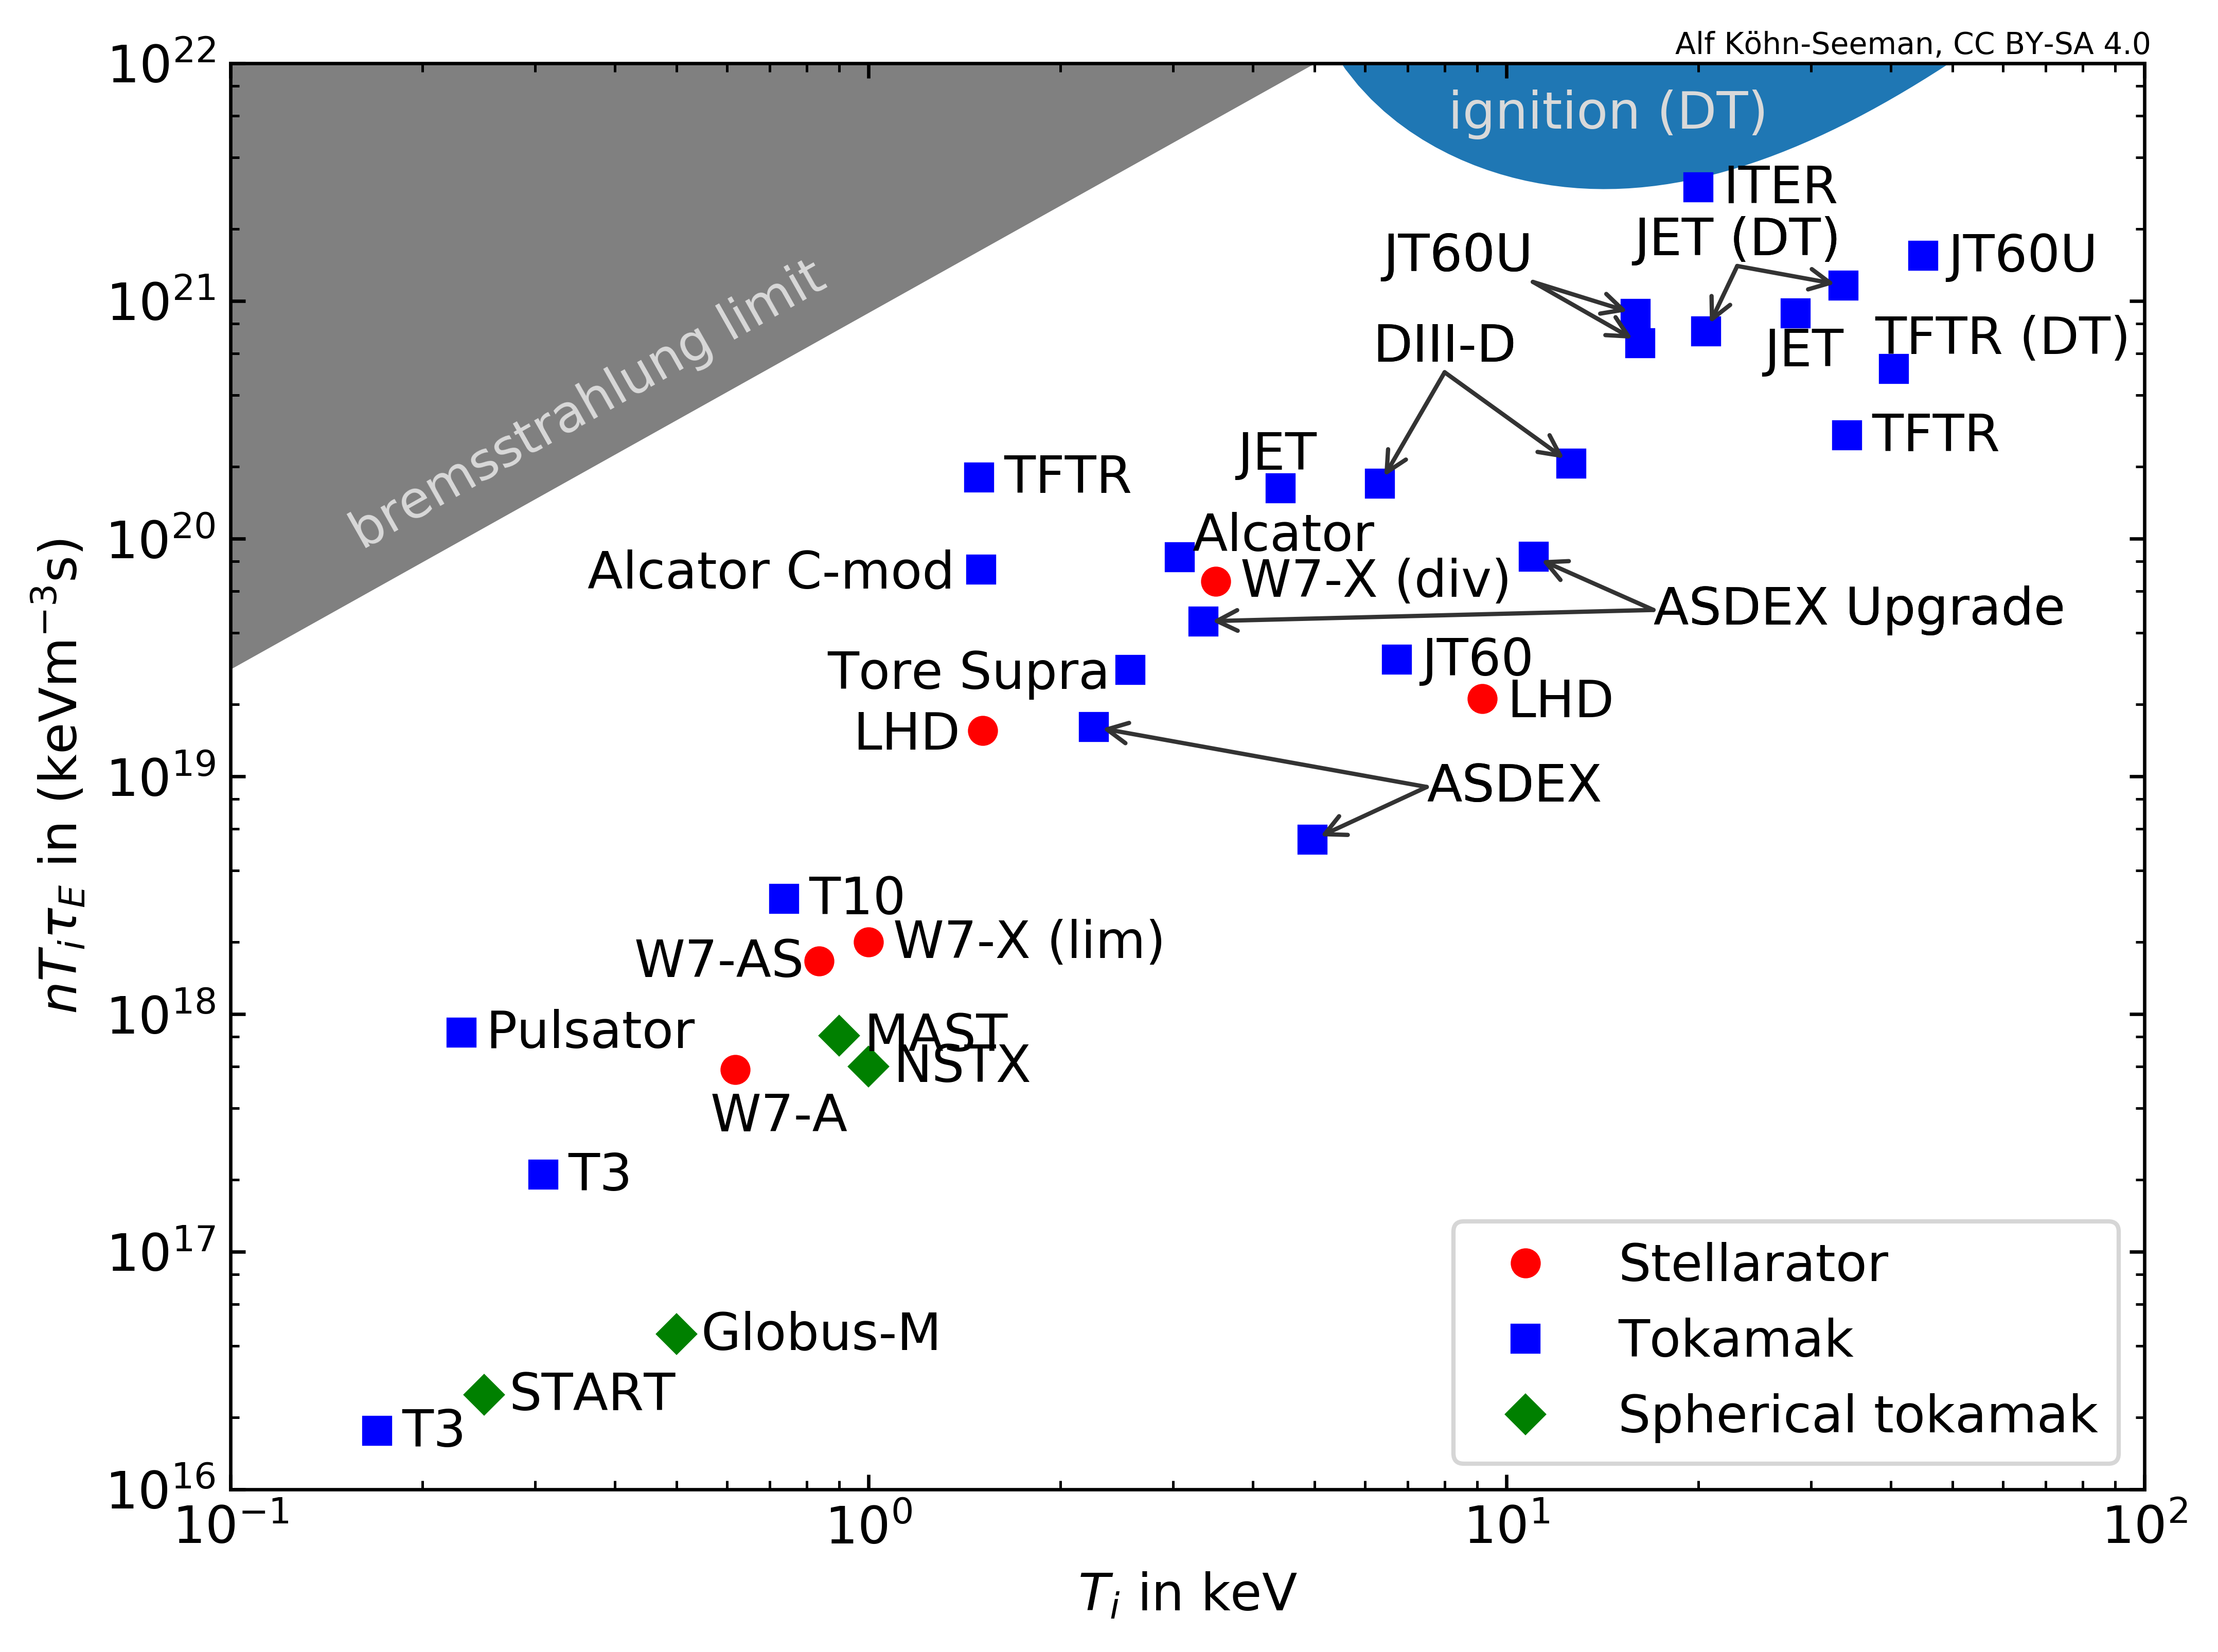
\includegraphics[width=1.0\textwidth]{figures/chap1/nTtau_machines.png}
		\caption{triple-product $n T_i \tau_E$ as a function of ion temperature $T_i$ for various devices (including stellarators, tokamaks, spherical tokamaks). Figure from \href{https://github.com/alfkoehn/fusion_plots/releases/tag/v1.0.0}{Alf Koehn}.}
		\label{fig:chap1:nTtau_machines}
	\end{center}
\end{figure}



% ####################################################
% ####################################################
% ####################################################
\section{Tokamak}
Sustaining a high temperature plasma in steady-state requires that the plasma be confined by magnetic field, such as in a tokamak, described in this section. The magnetic device called \emph{tokamak}, first developed in the Soviet Union in the early 1960s, is an efficient way to confine high temperature plasmas\sidecite{shafranov2001, azizov2012, mirnov2019}. It is an axially symmetric field configuration with a large toroidal magnetic field, a moderate plasma pressure and a relatively small toroidal current\sidecite[+0.4cm]{Freidberg2007}. By virtue of the highest achieved values of the $n T \tau_e$ product, tokamak is presently the leading magnetic configuration for a fusion reactor. Because of its performance, there is a large number of experimental tokamaks currently in operation or being constructed\marginnote{See \href{http://www.tokamak.info/}{www.tokamak.info} for an updated list of past, present and future experiments}. The following machines are cited in this manuscript: WEST (previously Tore-Supra, Cadarache, France), JET (Culham, UK), ASDEX-Upgrade (Garching, Germany), EAST (Hefei, China), HL-2A (Chengdu, China), KSTAR (Deajon, Korea) and the international project ITER (Cadarache, France).

\begin{marginfigure}[0cm]
	
\includegraphics[width=1\linewidth]{figures/chap1/tokamak_toroidal_field}
	\caption{Toroidal magnetic field produced by toroidal field coils.}
	\label{fig:tokamak_toroidal_field}
\end{marginfigure}

\begin{marginfigure}[0cm]
	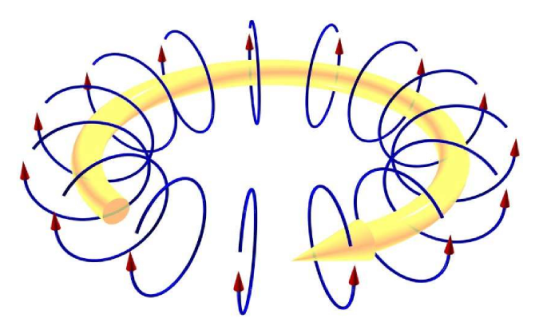
\includegraphics[width=1\linewidth]{figures/chap1/tokamak_poloidal_field}
	\caption{Poloidal magnetic field produced by the plasma current.}
	\label{fig:tokamak_poloidal_field}
\end{marginfigure}

\begin{marginfigure}[0cm]
	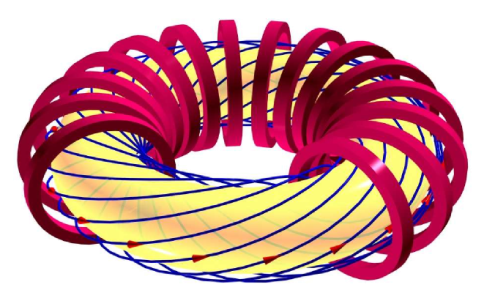
\includegraphics[width=1\linewidth]{figures/chap1/tokamak_helical_field}
	\caption{Helical magnetic field produced by the combination of toroidal and poloidal fields.}
	\label{fig:tokamak_helical_field}
\end{marginfigure}

In a tokamak, the plasma is confined by the combination of two magnetic fields: the toroidal and the poloidal fields. The toroidal field is the strongest one and is created in the toroidal direction by external "toroidal" field coils (Fig.\ref{fig:tokamak_toroidal_field}). Another set  of  external  coils, the poloidal field coils, which includes the central solenoid coils and additional control coils, are located concentric with the toroidal vacuum vessel.

An electric field in the toroidal direction is induced through the plasma by ramping a current in the central solenoid, like an electrical transformer in which the plasma acts as the secondary winding. This electric field induces a current in the plasma, current which creates the poloidal field (Fig.\ref{fig:tokamak_poloidal_field}). Poloidal and toroidal add up to form a twisted helical field (Fig.\ref{fig:tokamak_helical_field}) and both are required to confine the plasma into the vacuum vessel. 





%%%%%%%%%%%%%%%%%%%%%%%%%%%%%%%%%%%%%%%%%%
%%%%%%%%%%%%%%%%%%%%%%%%%%%%%%%%%%%%%%%%%%
\subsection{Ohmic Heating and Current Drive}
%%%%%%%%%%%%%%%%%%%%%%%%%%%%%%%%%%%%%%%%%%
\subsubsection{The Need for Additional Heating}
\marginnote{Parts of this section are taken from the "Tokamak dimensioning" activity given to French Master students in the frame of the "Master Fusion" and published in \citeauthyear{sarazin2019}.}

The plasma current density $J_p$ ($[\si{A/m^2}]$) flowing through plasma with resistivity $\eta$ ($[\si{\Omega.m}]$) heats up the plasma and generates an Ohmic heating power density $p_\Omega$:

\begin{equation}\label{eq:ohmic_power_density}
p_\Omega = \eta \; J_p^2 \;\; \si{[W/m^3]}
\end{equation}

where $\eta$ is the classical (parallel) Spitzer resistivity \cite[Eq.(11.15)]{Freidberg2007}:

\begin{equation}\label{eq:Spitzer_resistivity}
\eta
%= 0.51 \frac{\sqrt{2} e^2 m_e^{1/2} }{12 \pi^{3/2} \varepsilon_0^2 T_e^{3/2}} \ln \Lambda
\approx
3.3 \times 10^{-8} / \hat T^{3/2}  \, \mathrm{[\Omega.m]}
\end{equation}


Assuming homogeneous temperature in the plasma volume $V$, the Ohmic power $P_\Omega$ is:

\begin{equation}\label{eq:ohmic_power}
P_\Omega
=
3.3 \times 10^{-8} \frac{ I_p^2 }{ \hat T^{3/2} } V
\end{equation}

Since $\eta$ is proportional to $\hat T^{-3/2}$, $\eta$ decreases with increasing temperature and the role played by the Ohmic heating (\ref{eq:ohmic_power}) gradually becomes less important. 


The maximum temperature achievable using only Ohmic heating can be deduced from a 0D approximation by equalling Ohmic power input (\ref{eq:ohmic_power}) and losses (\ref{eq:losses}). Keeping only thermal losses and assuming homogeneous and equal density and temperature between ions and electrons, the plasma energy reads: 

\begin{equation}\label{eq:plasma_energy}
W 
= \int \frac{3}{2} k_B (n_e \hat T_e + n_i \hat T_i) \diff V 
=
 3 n \hat{T} V
\end{equation}

The confinement time $\tau_e$ in L-mode\sidenote{L-mode is the relevant mode here, since H-mode have mostly been achieved using a high fraction of external heating power.}) can be fitted from experimental results \cite[Eq.(14.155)]{Freidberg2007}:

\begin{equation}\label{eq:tau_e_modeL}
\tau_{e,L}
=
0.048  I_p^{0.85} R^{1.2} \kappa^{0.5} \hat n^{0.1} B^{0.2} A^{0.5} P_\Omega^{-0.5}
\end{equation}  
%which can be reexpressed as:
%$$
%\tau_L
%=
%0.037  
%\frac{\varepsilon^{0.3}}{q_\star^{1.7}}
%\frac{a^{1.7} \kappa^{1.7} \hat B^{2.1} A}{n_{20}^{0.8} T_k}  
%$$

At equilibrium, Ohmic power balances thermal losses\sidenote{Radiation losses are again neglected here for the sake of simplicity.} and the Figure~\ref{fig:ohmicpowervsthermallosses} shows that for typical tokamak fusion reactor parameters\sidenote{Main dimensions used:
\begin{itemize}
	\item $a$ = 2 m
	%\item $\varepsilon$ = 0.4
	\item $\kappa$ = 2
	\item $B$ = 4.7 T
	\item $n_{20}$ = 1.5 [$\times 10^{20}$ $\si{m^{-3}}$]
	%\item $q_\star$ = 2
	\item $A$ = 2.5 (average mass number DT mixture)
\end{itemize}
}
the maximum temperature achievable by ohmic heating is about few keV only. This temperature is not high enough for the alpha power to dominate: some other form of external heating is thus required. 

\begin{figure}[h]
	\centering
	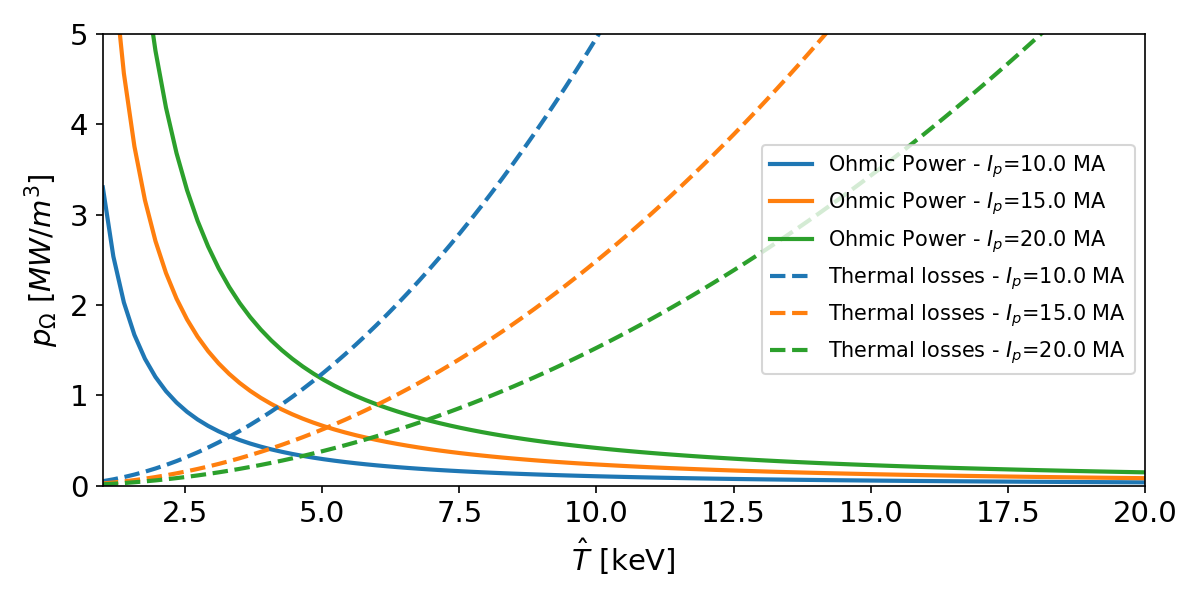
\includegraphics[width=1\linewidth]{figures/chap1/OhmicPower_vs_ThermalLosses}
	\caption{Ohmic Power Density and Thermal Losses as a function of the plasma temperature.}
	\label{fig:ohmicpowervsthermallosses}
\end{figure}


%%%%%%%%%%%%%%%%%%%%%%%%%%%%%%%%%%%%%%%%%%
\subsubsection{The Need for Non-Inductive Current Drive}
Operating a tokamak in steady-state conditions means sustaining a constant current into plasma (Fig.\ref{fig:tokamak_transformer_effect}). However, inducing a constant plasma current requires ramping the current in the central solenoid, which can't be done indefinitely. The duration is limited by the magnetic flux (number of Volt-seconds) that can be provided by the central solenoid coil. So, tokamaks are intrinsically pulsed machines.
Thus, to run in steady-state, a tokamak requires the plasma current to be sustained by other non-inductive means, ie. "non-inductive" current drive. Current-drive methods such as by high-power radio waves also heat the plasma, but not all heating methods generate substantial plasma current density. 

\begin{marginfigure}[-3cm]
	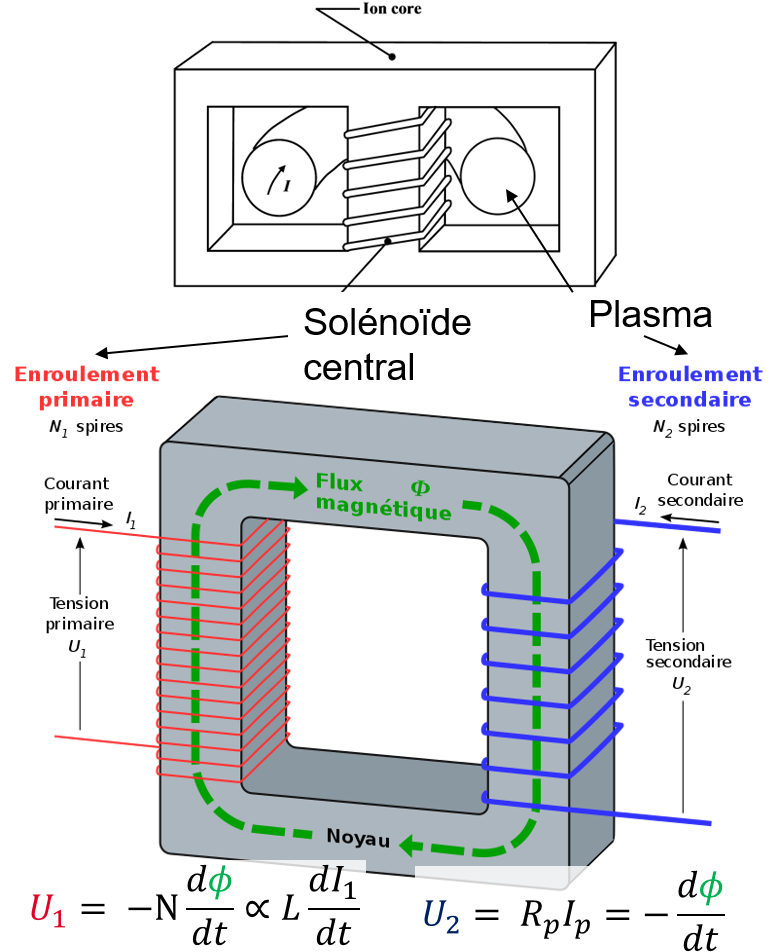
\includegraphics[width=1\linewidth]{figures/chap1/tokamak_transformer_effect}
	\caption{Tokamak transformer effect.}
	\label{fig:tokamak_transformer_effect}
\end{marginfigure}

\todo{Improve this section. Discuss RF CD efficiency}

%%%%%%%%%%%%%%%%%%%%%%%%%%%%%%%%%%%%%%%%%%
%%%%%%%%%%%%%%%%%%%%%%%%%%%%%%%%%%%%%%%%%%
\subsection{Radio frequency Heating and Current Drive}
\marginnote{Parts of this section are taken from the chapter 2 of the IAEA Textbook of Fusion Technology \citeauthyear{hillairet2020-1}}

%%%%%%%%%%%%%%%%%%%%%%%%%%%%%%%%%%%%%%%%%%
\subsubsection{General Principles}
As introduced in the previous section, auxiliary heating techniques are mandatory in tokamaks to raise ion temperature to the required values for burning state due to the physics inherent limitations. Several auxiliary heating and current drive systems have been developed in the history of fusion experiments and two broad types are used, namely neutral beam injection and radio-frequency methods. %Each has physics-based and technological strengths and weaknesses. 
The former involves  injection of high energy beams of neutral atoms which can cross the machine magnetic field and transfer its energy to the plasma via charge exchange reactions. Among the latter, many concepts have been tested\footnote{To the author knowledge, there is unfortunately no reference book listing all these various efforts and their associated successes (or failures). Putting apart the textbook dealing with waves in plasma, only few books have been written years ago specifically on the topic of RF heating and current drive: \citeauthyear{granatstein1985}, \citeauthyear{Golant1989}, \citeauthyear{Cairns1991}. Unfortunately, neither describes the technological aspects associated to a given heating or current drive method. Engineering "tips and tricks" and technological know-how is mostly transmitted internally in research institute with relatively few international exchanges. This was not a problem as the number of staff was sufficient. As cost-driven management results in staff reduction, this know-how tends to disappear... To sum up, there currently no "how to build a fusion plasma heating and current drive system" book (yet?).} and results reported in conferences and journal papers \sidecite{hwang1981, bers1984, england1989, jacquinot1999, pinsker2001} or in book chapters \cite[§6]{kikuchi2012}, \cite[§15]{Freidberg2007} or \cite{hillairet2020-1}. 

As the sizes of the fusion machines increased, a selection occurred on the kinds of selected RF systems, constrained by cost considerations, the know-how of the time and of course by the experience of people in charge\footnote{"L'histoire est juste peut-être, mais qu'on ne l'oublie pas, elle a été écrite par les vainqueurs", Alexis de Saint-Priest - 1842. "What is history but a fable agreed upon?" (Napoleon Bonaparte).}. Nowadays, the RF systems used in large fusion experiments are Ion and Electron Cyclotron Resonance Heating (ICRH and ECRH) and Lower Hybrid Current Drive (LHCD). Only ICRH and ECRH are planned in ITER\sidenote{\url{www.iter.org/mach/Heating}} after that LHCD has been removed from its latest research plan \cite{iterorganization2018}. 

All RF heating and current drive methods share the same following requirements:
\begin{enumerate}
	\item High Power RF generators, that transform electrical power into electromagnetic power
	\item Transmission Lines to transport the electromagnetic power to the antennas
	\item Antennas to couple the electromagnetic power to plasma waves
	\item Wave propagation and absorption on ions or electrons by wave-particle interactions
\end{enumerate}

Since the transmission lines are pressurized with an inert gas (or dry air) to increase breakdown voltage limits, one or more feed-through (or "windows") are therefore required before connecting them to an antenna inside the vacuum chamber. These components are made of ceramics or diamond, transparent to the RF waves but insuring the tightness between pressurized and vacuum regions. Windows for LHCD are discussed in Section~\ref{sec:RF_windows}.

In this manuscript, we will focus only on ICRH and LHCD systems. Moreover, we will not address the problems arising from the interactions between these two systems, when they are used either sequentially or simultaneously.



%%%%%%%%%%%%%%%%%%%%%%%%%%%%%%%%%%%%%%%%%%
\subsubsection{Ion Cyclotron Resonance Frequency}
The resonance between the natural cyclotron motion of an ion in a static magnetic field with an electromagnetic wave having the same (gyro)frequency have been recognized early in the magnetic fusion research as a bulk plasma heating method\sidecite[-1cm]{berger1958, stix1958}. Experimental confirmations rapidly confirmed the theoretical findings\sidecite{stix1958-1, stix1960, hooke1961, rothman1969}. Nowadays, ICRH is the RF heating scheme whose highest powers have been coupled, with for example up to 16.5~\si{MW} in JET \sidecite[+1cm]{jacquinot1999}. ICRH is used in almost all present day tokamaks at multi-\si{MW} level and it is likely it will  play an important role in next generation experiments and fusion reactors.

Hot plasmas being weakly collisional, FR waves damping have to rely on collision-less wave-particle mechanisms. 

Absorption of the ICRF wave power in the ion cyclotron range of frequency
can happen by three mechanisms: minority heating, harmonic heating or mode
conversion. 

The physical heating mechanisms at play at the ion cyclotron resonance is not as evident as the naming seems to imply. They are reviewed in much more details in \sidecite{perkins1984, becoulet1996}. In a single species plasma, the plasma wave which is used to propagate the RF power from the edge to the plasma centre has two possible circularly polarized components. One is rotating in the direction of the cyclotron rotation of the ions and one rotating in the direction of the electrons. A rotating ion sees in its frame of reference a constant electric field that can accelerate (or decelerate) it, depending on the phase of the electric field (i.e. its direction) with respect to the instantaneous speed of the ion\sidecite{Freidberg2007}. However, at the location of the resonance, the amplitude of the former component whose electrical field is rotating is the direction the ions vanishes and no absorption occurs. 

Fusion scientists then have discovered that inside the plasma, the polarization of the wave is mainly set by the dominant species, while the absorption depends on the resonant species. If the dominant species is different from the resonant species, then the component of the wave with the right polarization at the resonance (of the resonant species) is different from zero. Once absorbed, the minority species then transfers its energy to the bulk plasma by Coulomb collisions. This method is called \textit{minority heating} \sidecite{perkins1984} and is one of the most used in tokamaks\cite{jacquinot1999}. For example in most Tore Supra/WEST scenarios, plasma consists in deuterium (D) as a majority specie, with few percent in ratio of hydrogen (H) as a minority species\sidecite{bourdelle2015}. 

It is also possible to use higher harmonics of the cyclotron resonance to heat the plasma ions, i.e. $\omega = N \Omega_{ci}$ with $N$ an integer larger than 1. This method is called \textit{harmonic heating} and actually was combined with minority heating since the beginning of ICRH experiments\sidecite{jacquinot1977, hosea1979}. The theoretical analysis shows that good accessibility persists and that a reasonable portion of the wave has the proper in-phase polarization for strong wave–particle resonance. However, the damping rate depends sensitively on temperature and density and thus is not as robust and reliable as one might like\cite{Freidberg2007}. 

Power can also be absorbed directly by the electrons by Landau damping/Transit Time Magnetic Pumping or linear mode conversion to Ion
Bernstein Waves (IBW) \sidecite{stix1965, brambilla1985}. Recent developments use a combination of three ions to integrate a minority heating with mode conversion scenarios. A mix of two majority ions leads to a mode conversion layer where the amplitude of the electric field of the wave with the right polarization is increased. Locating this layer at the position of the resonance of a third, minority species can lead to strong absorption by this minority and highly accelerated ions\sidecite{ongena2017}.

Despite its relative good performances\sidecite{steinmetz1987}, ICRH is also known to have detrimental effects, among them the generation of metallic impurity in the plasma\sidecite{adam1987, noterdaeme1993, perkins1989}. As radiative losses ($P_{\mathrm{rad}}$ in Eq.\ref{eq:losses}) goes as the square of the electric charge of the ions, heavier metals impurity strikes the fusion power budget more than light elements. This problem of impurities had been solved in previous experiments by the use of graphite limiters and carbon-coated metallic surfaces. However, due to gas retention issues, these materials can't be used in future fusion reactor and plasma facing components equipping the experimental devices have been progressively changed to metallic ones, highlighting the impurity problem again\sidecite{ongena2017}.

Ion cyclotron was used to be promoted as the "cheapest" RF scheme since it has the advantage of operating in a frequency range where high power sources were readily available for MF to VHF frequency bands. However, this assertion should be moderated. As bandwidth demand led to an increase of the frequencies (which comes with higher propagation losses, leading to shorter ranges and more sources), the demand for high power transmitters tubes has been progressively converted to low power semiconductor amplifiers. Only a few high power vacuum tube manufacturers now remains, offering services that cannot always be described as "cheap".


%%%%%%%%%%%%%%%%%%%%%%%%%%%%%%%%%%%%%%%%%%
%%%%%%%%%%%%%%%%%%%%%%%%%%%%%%%%%%%%%%%%%%
\subsubsection{Lower Hybrid Resonance Frequency}
Originally, the occurrence of a wave resonance, the \emph{lower hybrid resonance}, has been anticipated to lead to strong wave-particle interaction through linear and non-linear mode conversion to a hot plasma wave\sidecite{stix1992}. With an appropriate RF launcher conceived to excite cold plasma waves, these would propagate into the plasma until reaching the lower hybrid resonant layer at $\omega_{LH}$. This resonance exists in tokamak plasma in the region close to the ion plasma frequency $\omega_{pi}/2\pi$, which lies in the lower end of the microwave band (1-5~GHz). At this layer, the perpendicular group velocity vanishes and the waves can convert into a hot plasma mode which is absorbed. This heating technique, known as \emph{Lower Hybrid plasma Ion Heating} (LHIH) or \emph{Lower Hybrid Resonance Heating} (LHRH), was the originally experimentally investigated method in the 70'\sidecite{bellan1974, hooke1972, golant1972, tonon1977}. Different physical mechanisms have been invoked to explain the energy absorption, such as stochastic Ion Heating in \citeauthyear{karney1978} and quasi-linear electron Landau damping in \citeauthyear{brambilla1983}.


In the 80', effective ion heating had only been obtained in a small number of experiments and research along the application of LH waves towards bulk ion heating were slowing down\sidecite{gormezano1986, porkolab1984, tonon1984}. The reason for this is that bulk ion heating near the mode conversion layer appeared to be less reproducible and more difficult to achieve than electron heating. Indeed, as the wave frequency gets closer to the lower hybrid frequency, the shorter wavelength waves may be more effectively absorbed and/or scattered near the plasma surface by non-linear effects such as parametric instabilities, low-frequency fluctuations, etc. Moreover, for LH bulk ion heating, the unconfined ions impinging on the wall induced a large amount of metallic impurities and then the increase of power radiated by the plasma.

Rather than trying to heat ions, it was theorized postulated that high phase velocity waves travelling in the direction parallel to the magnetic field could interact quasi-linearly by Landau interaction with the electrons population, and, by using an asymmetric spectrum could drive a large amount additional of toroidal plasma current \sidecite{fisch1978}. In the same fashion that for LHRH, the RF power is coupled to the plasma via launchers made of rectangular waveguides stacked periodically in the horizontal direction parallel to the toroïdal magnetic field. However, at the contrary of LHRH launchers, the LH waves are launched preferentially in one toroidal direction by mean of a phased array. The LH wave excited by such an array has an asymmetric parallel spectrum. The LH waves create an asymmetry in the electron distribution, which ultimately results in a net electric current \sidecite{fisch1987}. This technique is known as \emph{Lower Hybrid Current Drive} and despite the fact that the Lower Hybrid resonance is not any more involved in the use of this method in tokamaks, the term remained. LHCD has been confirmed on the PLT tokamak in 1982 \sidecite{bernabei1982} and in Alcator-C in 1984 \sidecite{porkolab1984}. 

Since in 1982 many impressive results were presented on LHCD\sidecite{stevens1983, porkolab1984, tonon1983} toward steady state or quasi steady state tokamak operations, most LH experiments were dedicated to electron interaction and especially to current drive. A recent review of LHCD is available in \sidecite[+0.5cm]{bonoli2014}.

\marginnote[+1cm]{These terms will be explained in Section~\ref{sec:waves-in-plasma}.}
Currently, the "LH waves" term refers to the waves which satisfy the slow-wave branch of the cold plasma dispersion relation for parallel index larger than one ($|n_{\parallel}|>1$) and a RF frequency $\omega$ which lies between the ion cyclotron $\omega_{ci}$ and the electron cyclotron $\omega_{ce}$ frequencies. 

%For the LH method which operates at the lower end of the microwave band (1-5 GHz) klystrons transform electrical power into electromagnetic power (step 1), which is transported to the plasma using waveguides (step 2). The power is coupled to the plasma with antennas called "grills" because of their characteristic shape (step 3), transported inside the plasma by plasma waves (typically the slow wave) (step 4), and absorbed on ions or electrons by wave-particle interaction (step 5).


\subsubsection{High Power RF Sources}
\todo{add some pictures}
In the ICRH frequency range (30-60~\si{MHz}), electrical to electromagnetic power transformation is typically carried out by a series of amplifiers (Tetrode, Triode), a technology derived from high-power, steady-state broadcast transmitters. Typical unit sizes for present ICRH pulsed systems are 2~\si{MW} (around 500~\si{kW} in CW). The Tore Supra/WEST ICRH plant is equipped with Thales Electron Device tetrodes\sidecite{clerc1986, clerc1992-1} and shares some aspects of the JET ICRH plant which is detailed in \sidecite[+0.5cm]{wade1994}.

In the LHD frequency range (1-5~\si{GHz}) which lies close the lower end of the microwave band, the electromagnetic power is generated by klystrons. A klystron is a vacuum tube used as amplifiers at narrow band microwave and radio frequencies. In the fusion domain, they are used mainly to produce high power waves, at the level of hundred of kilo watts during many seconds. First klystrons have been invented by the Varian brothers in 1937 \sidecite{Pond2008}. The first klystrons have been intensively used during World War II, as RF power generators for RADAR systems. Klystrons sources between 2.45~\si{GHz} and 5~\si{GHz} are now available at the 0.5-0.8~\si{MW}/10-1000~\si{s} level. The Tore Supra/WEST system frequency is 3.7~\si{GHz}$\pm$ 2.5~\si{MHz} \sidecite{peauger2005, kazarian2005, beunas2009, delpech2011-1}),

% #####################################################
\subsubsection{Transmission Lines}
Many devices have been developed in order to transmit, measure, combine or split high RF power from one point to another. These devices are commonly used on ICRH and LHCD systems to transport the power from the sources to an antenna, but also in order to protect the sources from possible reflected RF power by the plasma.  

\todo{Add some pictures}

% #####################################################
% #####################################################
\subsubsection{High Power Coaxial Components}
Rigid coaxial transmission lines for high power application are commonly available in 30, 50 or 75~$\si{\Omega}$ characteristic impedances. The former is optimized for power handling while the later is used for minimum attenuation. In between, 50~$\si{\Omega}$ lines are a compromise between power handling and attenuation. 

\todo{Picture of coaxial components}

Rigid coaxial lines are used in the ICRH frequency range (30-60~\si{MHz}). These components are usually filled with dry air or nitrogen up to few atmospheres in order to avoid dielectric voltage breakdown. Coaxial lines main properties are recalled in Section~\ref{sec:coaxial_lines}.

In Tore Supra/WEST, ICRH lines consist in Spinner 30~\si{\Omega} 9" coaxial lines ($\phi_\mathrm{i}/\phi_\mathrm{o}=140/230~\si{mm}$ with 2 and 5~\si{mm} thickness respectively). The inner conductor is often made of copper for the internal conductor while the outer conductor is made of aluminium AG5. Long pulse duration can be limited by the thermal expansion of the (inner) conductor. Modelling have shown that forcing dry air or nitrogen flow between inner and outer conductor would however be sufficient to reach 2\si{MW}/1000\si{s} \sidecite{vulliez2005}.

As the RF frequency increases, coaxial cable losses become unpracticable for high power applications. In the LH range of frequencies (1-5~\si{GHz}), hollow rectangular waveguides are preferred for the transport of the RF power from the klystrons to the torus. In addition to their low losses, they also allow a greater breakdown voltage than coaxial lines of the same size. In this frequency range the wavelength in vacuum is of the order of 30~\si{cm} to 6~\si{cm}. Rectangular waveguide main properties are recalled in Section~\ref{sec:rectangular_waveguide}

In both cases, since the lines are connected to the antenna (which is in vacuum), a barrier is required in the
line to separate the pressurized part of the line from the vacuum part of the line. This is done with a \textit{feed-through} (or \textit{window}), a ceramic piece that provides the sealing barrier function. These device must be as transparent as possible for the RF, that is not change the characteristic impedance of the line at that point nor induce reflection or reduce its voltage stand-off capability. Coaxial line feed-through for ICRH are usually done a conical piece of ceramic (alumina) brazed or assembled to the central and outer conductors of the transmission line. The dimensions of those conductors are varied to keep the characteristic impedance of the line constant as the ceramic would modify this characteristic impedance if the dimensions of the line would stay the same. For LHCD, A window consists in a dielectric medium inserted between two rectangular waveguides. The dimensions of the dielectric medium (a ceramic, such as beryllium oxide BeO or alumina) are calculated not to produce reflected power. Since part of the power is always absorbed in the ceramic, great care is applied to correctly cool the window to avoid heating the ceramic which could make it break. The Section~\ref{sec:RF_windows} is dedicated to LH windows.


% #####################################################
% #####################################################
% #####################################################
\subsubsection{Antennas}\label{sec:RF_antennas}
\marginnote{In the litterature, the terms \textit{launchers} or \textit{couplers} are sometime used in the fusion community to distinct LHCD antennas from ICRH antennas. In this document, we do not make any difference between these terms, they are all radiating elements. }

Being inserted in machine's ports, ICRH and LHCD antennas are facing the plasma and therefore must  withstand harsh operational constraints: 
\begin{itemize}
	\item high vacuum compatibility ($<10^{-4}\,\si{Pa}$, 
	\item high temperature (above 150°C during machine baking)
	\item high heat fluxes on plasma facing components (up to few \si{MW/m^2} transiently or in steady-state conditions)
	\item high RF power (Megatwatt range, CW power), inducing large RF losses
	\item large electromechanical forces and torques induced by disruption, ie. brutal loss of plasma (\si{MN})
\end{itemize}
These constraints restrict the list of usable materials to certain kinds of metals or ceramics only. Moreover, the large heat fluxes due to the plasma or to the RF losses require the antenna to be actively cooled in order to sustain continuous operation. Moreover, in future machine like ITER, neutron activation and nuclear safety and remote handling compatibility  add supplementary constraints on material choices and mechanical designs.

In this manuscript, only IC and LH antennas are discussed. Despite that IC antennas can be used for current drive and LH power are heating plasma, these systems will be regarded as dedicated to plasma heating and current drive respectively. ICRH antennas and in particular the WEST antenna are discussed in Section~\ref{sec:ICRH_antennas}. The Tore Supra/WEST and ITER LHCD antennas are discussed in Section~\ref{sec:LHCD_antennas}.


% #####################################################
\subsubsection{Waveguide Plumbing – a practical example with Tore Supra/WEST}
As an example of high power system, the Tore Supra/WEST LHCD system is illustrated in Figure \ref{fig:toresupralhcdsystem}. The power is generated at the klystron plant and transmitted to the two launchers through rectangular waveguides (8~lines per launcher). 

\begin{figure}
	\centering
	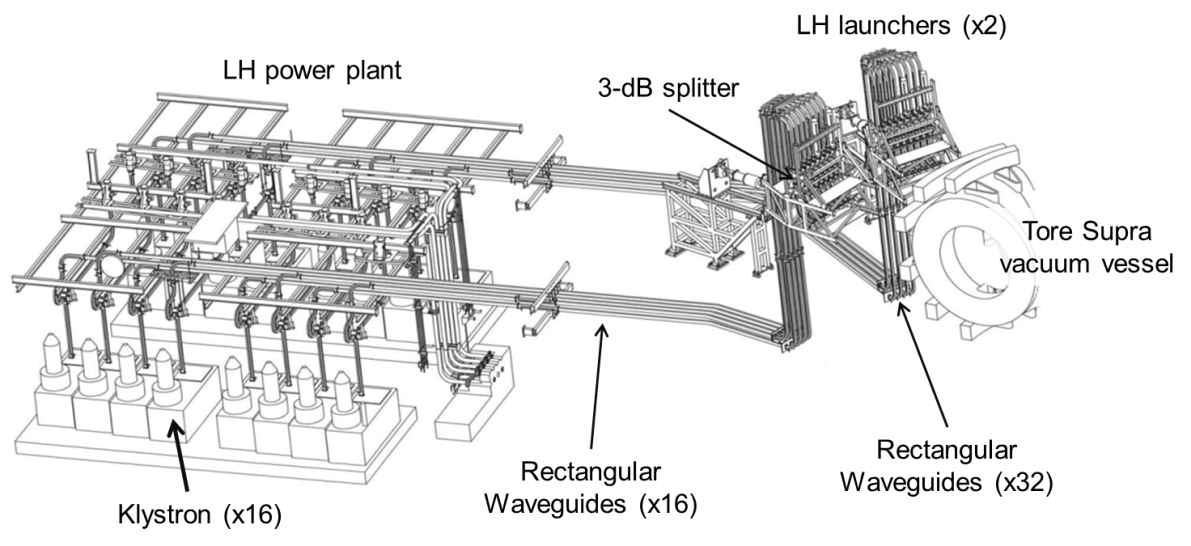
\includegraphics[width=0.9\linewidth]{figures/chap1/ToreSupra_LHCD_System}
	\caption{Schematic of the Tore Supra LHCD system, from the klystrons plant to the vacuum vessel.}
	\label{fig:toresupralhcdsystem}
\end{figure}

Once reaching the launcher rear end, the power goes trough a \textit{hybrid junction} (also called 3-dB splitter). This device splits the forward power into two waveguides, one to feed the upper part and the other for the lower part of the launcher.  If reflected power (from the plasma) returns from these two waveguides, the power is recombined and directed to a fourth one. An actively cooled water load is connected to this fourth port, in order to dump the remaining RF power reflected by the plasma and thus protect the klystron. A rectangular waveguide 3-dB splitter is illustrated in Figure \ref{fig:hybridjunction1}. 

\begin{figure}[h]
	\centering
	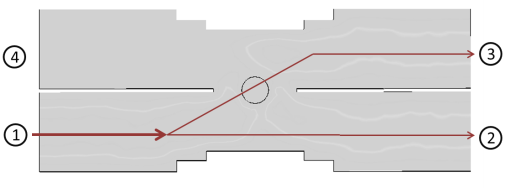
\includegraphics[width=0.4\linewidth]{figures/chap1/HybridJunction1}
	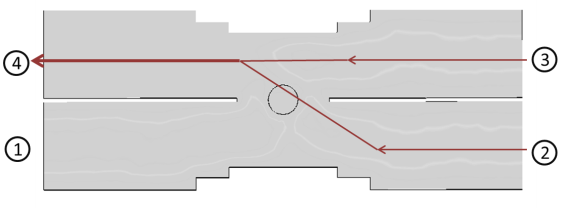
\includegraphics[width=0.4\linewidth]{figures/chap1/HybridJunction2}
	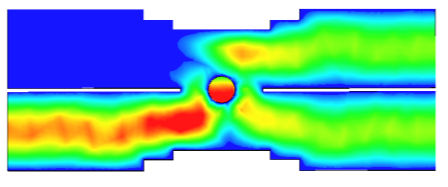
\includegraphics[width=0.4\linewidth]{figures/chap1/HybridJunction_Efield}
	\caption{Top: Illustration of an rectangular waveguide hybrid junction. When excited from port 1, the power is split to ports 2 and 3. when the power comes from ports 2 and 3, the power is recombined and directed to port 4, where the power is dumped into a water load. Bottom: The electric field distribution when excited from port 1. }
	\label{fig:hybridjunction1}
\end{figure}


After being split by the hybrid junction, the RF power goes through various devices up to the plasma (Figure \ref{fig:toresuprac4cad}): 
\begin{itemize}
	\item A bidirectional coupler, which allows measuring the forward and reflected power amplitude and phase ;
	\item A DC break, which isolates the DC potential of the tokamak from the DC potential of the transmission line (for the protection of persons);
	\item A vacuum feed-through (window) which isolates the tokamak vacuum from the pressurized medium existing in the waveguide. These windows (16 by launchers) are illustrated in Figure~\ref{fig:toresuprac4cad}. More details on windows are given in Section~\ref{sec:RF_windows}
	\item A $\TE_{10}-\TE_{30}$ mode converter, which splits the incoming RF power into three, thus leading to split the power into three poloidal rows of waveguides. A mode converter is a rectangular waveguide device which large side is modulated in order to allow higher modes (such as $\TE_{20}$, $\TE_{30}$ and $\TE_{40}$) and such that the power is totally transferred from one mode to another one (efficiency is close to 100\%). Once the power is transferred to the $\TE_{30}$ mode, metallic septa located in zero field regions split the power into three independent waveguides. The device is illustrated in Figure~\ref{fig:modeconverter}. More details on $\TE_{10}-\TE_{30}$ mode converter are given in Section~\ref{sec:mode_converter}
	\item Finally a multijunction antenna, a structure which will be described in details in the Section~\ref{sec:multijunction}, splits and phases the power in the toroidal direction before leaving the antenna to the plasma. 
\end{itemize}


\begin{figure}
	\centering
	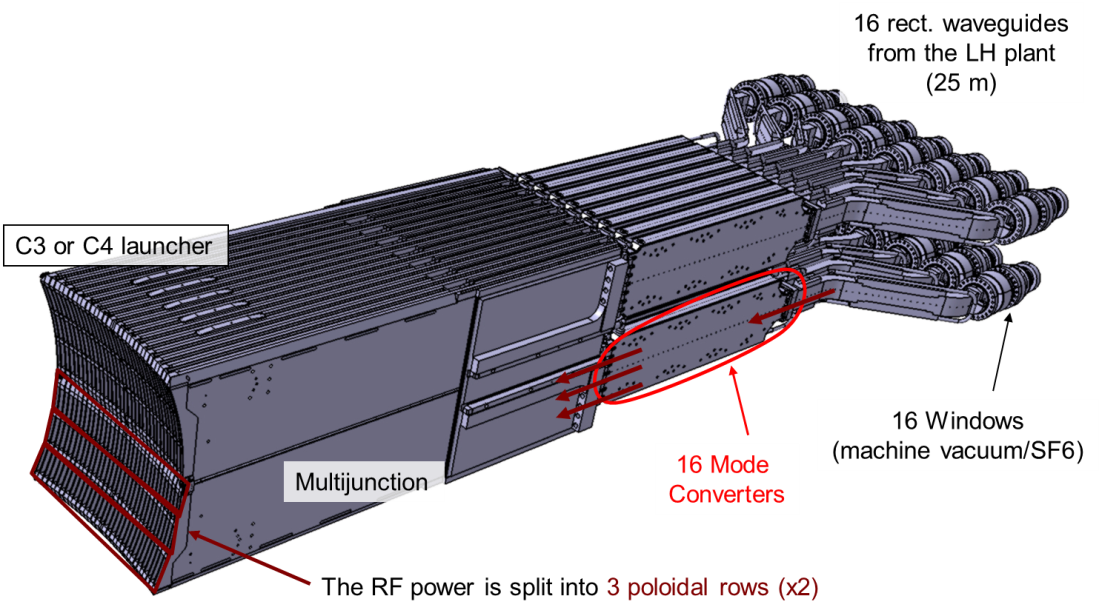
\includegraphics[width=0.9\linewidth]{figures/chap1/ToreSupra_C4_CAD}
	\caption{Illustration of the power splitting scheme in WEST LHCD launcher LH1 or LH2.}
	\label{fig:toresuprac4cad}
\end{figure}


\begin{figure}
	\centering
	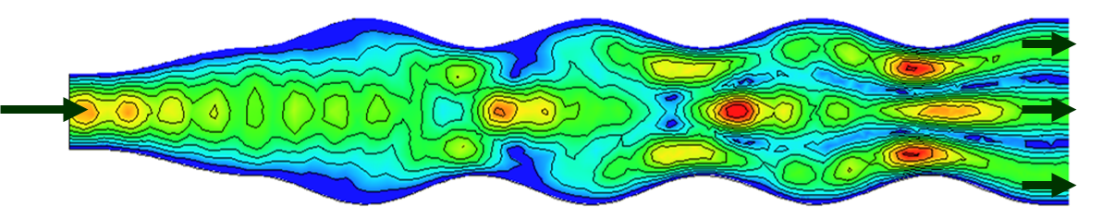
\includegraphics[width=0.9\linewidth]{figures/chap1/ModeConverter}
	\caption{Illustration of the electric field distribution in a TE10-TE30 mode converter at 5 GHz. The device is excited from the left.}
	\label{fig:modeconverter}
\end{figure}
